\chapter{Как из поля на сетке получить прогноз}
\label{primer:chapter}

\section{Одна задача и одно поле}
\label{primer:physical}
Представьте, что через неоднородную среду проходит плоская волна.
Мы знаем свойства среды и можем менять направление волны.
Для каждого направления нас интересует одно и то же: каким будет
рассеянное поле в каждой точке области? Один расчёт методом конечных
элементов даёт поле для одного набора условий. Серия таких расчётов
даёт примеры, по которым можно учиться предсказывать следующее поле.

Обозначим набор условий через $p=(A,n,k,\theta)$. Функции $A(x)$ и $n(x)$
задают свойства среды, $k>0$ задаёт волновое число, а $\theta$~--- угол
падения в радианах. Координата $x=(x_1,x_2)$ отвечает на вопрос «где?»,
а набор $p$~--- «при каких условиях?». Если взять две точки при одном $p$,
мы увидим разные значения одного поля. Если изменить $p$ и оставить точку
на месте, получим значение другого поля.

\begin{center}
\begin{tabularx}{\linewidth}{@{}l X@{}}
\toprule
Поле & Как его получить \\ \midrule
Падающее $u_i$ & Вычислить по формуле $u_i(x)=\exp(\ii k\,d\cdot x)$,
где $d=(\cos\theta,\sin\theta)$ и $\ii^2=-1$.\\[2pt]
Рассеянное $u_s$ & Решить краевую задачу или получить приближённый
прогноз обученной модели. Это поле изучается в пособии.\\[2pt]
Полное $u_{\rm tot}$ & Сложить поля как комплексные числа:
$u_{\rm tot}=u_i+u_s$.\\
\bottomrule
\end{tabularx}
\end{center}

Метод конечных элементов (МКЭ, англ.\ FEM) заменяет искомую
функцию набором чисел на сетке. Для линейных треугольных элементов
это значения в узлах $U_i=u_{s,h}(x_i)$, где $h$ характеризует размер
элементов. По ним поле восстанавливается и между узлами:
\[
  u_{s,h}(x)=\sum_{i=1}^{N} U_i\,\varphi_i(x).
\]
Функция $\varphi_i$ равна единице в своём узле и нулю во всех остальных.
Внутри треугольника поле линейно интерполирует значения в трёх вершинах.

\begin{idea}{Какие данные будем разбирать}
В эталонном расчёте GMsFEM область $[-2,2]^2$ содержит 24 включения.
На фоне $A=n=1$, внутри включений $A=0{,}2$ и $n=10$.
В сетке $53\,246$ узлов и $105\,690$ треугольников.
Для этой фиксированной среды сеть по $k$ и $\theta$ предсказывает
50 чисел, по 25 на каждую компоненту комплексного рассеянного поля.
\end{idea}

\clearpage
\section{Как восстановить поле на одном треугольнике}
\label{primer:three-objects}\label{primer:example}
Возьмём тестовый расчёт №\,940 при $k\approx1{,}48616$ и $\theta\approx3{,}30401$.
На рисунке выделен треугольник №\,53227 с вершиной в начале координат.
Номера элементов и узлов соответствуют массивам Python с нумерацией от нуля.

\begin{center}
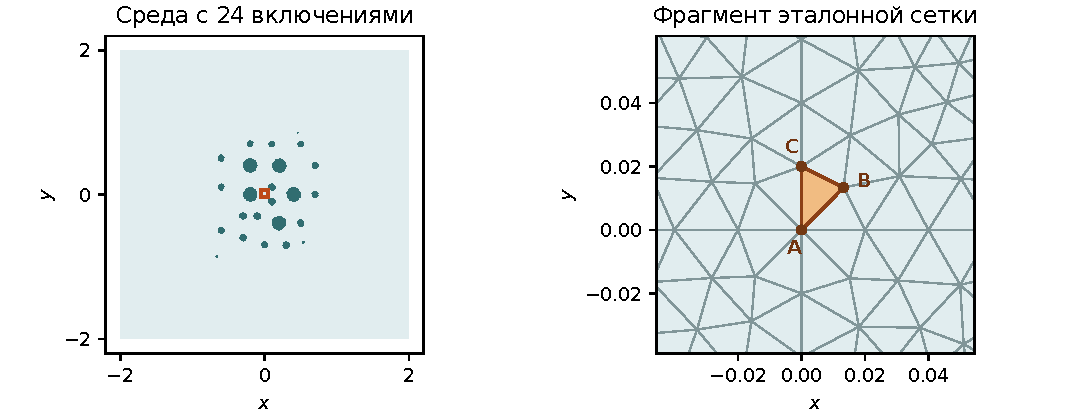
\includegraphics[width=.91\linewidth]{assets/notation_example.pdf}
\captionsetup{hypcap=false}\captionof{figure}{Эталонная геометрия GMsFEM.
Слева тёмным цветом показаны включения, рамкой отмечена область увеличения.
Справа видны рёбра сетки и вершины выбранного элемента.}
\label{primer:figure}
\end{center}

Один \emph{снимок} содержит значения поля сразу во всех узлах.
В каждом узле $i$ усредним действительную часть по 856 обучающим снимкам.
Получим среднее $\mu_i$. Пространственная \emph{мода} $\phi_j$ тоже имеет
значение в каждом узле, но задаёт форму отклонения от среднего.
Для нового запроса сеть выбирает один коэффициент $\widehat c_j$ на всю моду:
\[
 \widehat f_i=\mu_i+\phi_1(x_i)\widehat c_1+
                     \sum_{j=2}^{25}\phi_j(x_i)\widehat c_j .
\]

\begin{center}
\begin{tabular}{@{}lr r r r r r@{}}
\toprule
 & Узел & Среднее & Мода 1$\,\times\widehat c_1$ & Моды 2--25 & Прогноз & МКЭ\\
\midrule
$A$ & 27000 & $-0{,}21008$ & $-0{,}28392$ & $-0{,}04905$ & $-0{,}54305$ & $-0{,}54449$\\
$B$ & 26855 & $-0{,}21080$ & $-0{,}28662$ & $-0{,}03050$ & $-0{,}52792$ & $-0{,}52947$\\
$C$ & 26705 & $-0{,}21035$ & $-0{,}28694$ & $-0{,}04236$ & $-0{,}53966$ & $-0{,}54119$\\
\bottomrule
\end{tabular}
\end{center}

\textbf{Проверка строки $A$.} Сеть дала $\widehat c_1=-0{,}562294$,
а первая мода в этом узле равна $0{,}504940$. Их произведение
равно примерно $-0{,}28392$. Прибавьте среднее и вклад остальных мод:
получится $-0{,}54305$. Последний столбец таблицы получен независимым
способом: для тех же $k,\theta$ решена система МКЭ.

\clearpage
\section{Что известно при новом запросе}
\label{primer:stages}\label{primer:why-svd}
Как сеть получила одно число $\widehat c_1$ для всех трёх вершин?
Рассмотрим, какие величины вычисляют заранее и какие зависят от запроса.

\smallskip\noindent{\sffamily\bfseries\color{navy}1. Решить обучающие задачи}\par\nopagebreak[4]
Для каждого выбранного $p$ метод конечных элементов даёт вектор $U(p)$.
Для проверки качества откладывают отдельные группы данных. Например, при
проверке на новых частотах все направления одной частоты должны попасть
в одну и ту же часть выборки.
\smallskip\noindent{\sffamily\bfseries\color{navy}2. Найти пространственные моды}\par\nopagebreak[4]
По обучающим снимкам вычисляют среднее $\mu$ и матрицу мод
$\Phi=(\phi_1,\ldots,\phi_r)$. Каждая колонка~--- поле на всей сетке.
Такое представление даёт собственное ортогональное разложение
(англ.\ proper orthogonal decomposition, POD). Моды находят с помощью
сингулярного разложения матрицы данных (singular value decomposition, SVD).
При $r$ модах у каждого снимка $r$ коэффициентов.
\smallskip\noindent{\sffamily\bfseries\color{navy}3. Обучить модель коэффициентов}\par\nopagebreak[4]
Модель проекта основана на идее спектрального нейронного оператора
(spectral neural operator, SNO). В выбранном POD-базисе сеть с весами
$\omega$ переводит признаки запроса в коэффициенты
$\widehat c_j$. В ходе обучения $\omega$ меняют так, чтобы восстановленные
поля были близки к расчётным. Среднее поле и моды на этом этапе уже заданы.
\smallskip\noindent{\sffamily\bfseries\color{navy}4. Восстановить новое поле}\par\nopagebreak[4]
По новому набору $p$ сеть выдаёт коэффициенты. После отмены нормировки
выполняют сложение $\widehat f=\mu+\sum_{j=1}^r\phi_j\widehat c_j$.
В базовой модели так восстанавливают отдельно действительную и мнимую части:
$\widehat u_s=\widehat f_R+\ii\widehat f_I$.


\begin{worked}{Проверьте себя}
Изменим только первый коэффициент прогноза на $+0{,}1$. Как изменится
действительная часть поля в вершине $A$? А в других узлах?

\textit{Ответ.} В вершине $A$ добавится $0{,}1\cdot0{,}504940=0{,}050494$.
В каждом другом узле прибавка равна $0{,}1\phi_1(x_i)$. Таким образом,
у коэффициента одно значение на весь снимок, а изменение поля в разных
узлах определяется формой моды.
\end{worked}

В главе~\ref{math:fem} получим уравнение для узлового вектора $U(p)$.
В главе~\ref{math:pod} найдём моды по обучающим снимкам, а в
разделе~\ref{code:operator} разберём, какие матрицы действуют на
коэффициенты внутри нейронного оператора.
